\section{Experiments}\label{sec:exp}

This section \textbf{reports as results only what was actually measured}. The behavioral consistency, legibility, and per-cycle latency of the decision layer are \textbf{measured} with an offline harness that drives the actual decision core, and are presented in \cref{subsec:main,subsec:ablation} (ablation and $\rho$-sweep) and \cref{subsec:latency} (per-cycle latency); the harness setup and metrics are given in \cref{subsec:setup}, and the sensitivity-analysis design is given in \cref{app:sensitivity}. Performance metrics that require physical simulation or a real robot, the external baselines, and the user study were not measured and are therefore not presented as results; their protocols are specified in full, as a preregistration, in the Planned Evaluation of \cref{app:planned}. No measured value is fabricated.

\subsection{Experimental Setup}\label{subsec:setup}

\noindent\textbf{Harness and hardware.} The measurements in this section are obtained by driving the \textbf{actual decision core} (\code{DecisionCore}) with the \code{compass\_eval} offline harness across 5 reproducible encounter scenarios $\times$ 50 seeds $\times$ 6 variants ($dt = 0.05\,\text{s} = 20$ Hz, horizon 10 s; behavioral rerun CPU AMD EPYC 9V74; historical latency CPU AMD Ryzen 5 5500GT). All figures are computed deterministically from the decision stream, and the raw data (\code{compass\_eval/results/ablation\_raw.csv}) are released; \cref{tab:params} lists the default knobs used. What this harness measures is the decision layer's behavioral consistency, legibility proxies, and per-cycle latency; performance metrics that require physical simulation (success rate, collision rate, minimum social distance, lateral jerk) and the external baselines / user study are separated into the Planned Evaluation (\cref{app:planned}).

\noindent\textbf{Scenarios and comparators.} The scenarios are ambiguous tie (\code{near\_tie}), transient spike (\code{transient\_spike}), mid-course reversal (\code{mid\_reversal}), clean advantage (\code{clean\_commit}), and intermittent advantage (\code{intermittent}). The measured configurations and internal comparators are the proposed method (full) and $-$hysteresis ($\Dfloor = 0$), $-$progress hardening ($k_\rho = 0$), $-$accumulator (immediate argmin), \textbf{simple dwell} (a continuous 0.6 s dwell timer in place of leaky accumulation; comparison in \cref{subsec:leak}), and a \textbf{synthetic correspondence-loss stress comparator} (historical CSV key: $-$class correspondence). This last comparator randomly selects a label when $|J_R-J_L|<0.10$ and otherwise uses argmin; it also lacks the accumulator, so it is not an isolated removal of class correspondence from \sname. Immediate argmin and simple dwell are separate comparator policies, whereas only $-$hysteresis and $-$progress hardening are knob-only core ablations. The $-$safety-override variant is equivalent to the proposed method in offline scenarios that contain no safety event (its effect lies in the collision regime), so it is excluded from this measurement set; its evaluation belongs to the physical-simulation evaluation (\cref{app:planned}).

\noindent\textbf{Legibility proxy.} Legibility (time-to-legible) is computed by applying the \cref{subsec:observer} Bayesian observer to the decision stream, but because the offline harness has no realized trajectory, the observer here consumes the \textbf{per-cycle committed passing side (the decision stream) as a proxy observation} in place of the kinematic motion cues specified in \cref{subsec:observer}, using log-odds updates to avoid posterior saturation, with a symmetric misread likelihood parameter $\varepsilon$ --- an assumed observation error probability, not separately sampled corruptions of the stream ($\varepsilon = 0.2$, $p^* = 0.9$ in this measurement). This is an additional simplification of the \cref{subsec:observer} kinematic-cue observer (implementation: \code{src/compass\_eval/include/compass\_eval/harness.hpp:171-196}). Hence the offline $t_{\text{legible}}$ measures \textbf{the legibility of the decision stream}, not an independent axis of motion legibility; the kinematic-cue observer and human validation are left to the planned evaluation (\cref{app:planned}). The hold condition of the offline run is held-to-horizon-end, i.e., effectively $\Delta_{\text{hold}} = T - t$, the strictest possible hold condition, and additionally requires at least 0.30 s of observed follow-up after the first sample of that confident suffix. Final-tick or shorter-follow-up crossings are censored; these are the operational rules used for the corrected CSV. The illegibility rate is the fraction of trials in which the posterior never stabilizes above $p^*$ by the end of the trial (right-censored).

\noindent\textbf{Input and counting conventions.} The archived scenario generator supplies unclipped Gaussian perturbations directly to \code{step\_evals}; that distribution is not bounded almost surely. It is a scripted robustness experiment, not an empirical verification of P1/P2's bounded-input hypothesis or the normalized production-cost path. Bounded deterministic/property tests provide separate software checks. All six policy streams use the same switch-count convention $\sum_{i=1}^{n-1}[s_i\ne s_{i-1}]$: the initialized class to first emitted output is excluded for every policy. Thus an argmin choice of L on its first output in \code{clean\_commit} records zero subsequent transitions, not an absence of an initial decision. This boundary convention is retained for archived reproducibility and is distinct from the opportunity scorer's response-event accounting.

\noindent\textbf{Observer result versions.} The original main snapshot at \code{9fe495a} used probability-space updates. The log-odds-only observer change (PR~12, \code{5343d457}) fixes numerical saturation without adding a follow-up requirement. The current results additionally require 0.30 s of observed follow-up, a metric-definition change rather than merely a numerical fix. These versions must not be pooled. Source/input/configuration provenance and preserved historical values are recorded separately from the current corrected table; unchanged decision streams do not mean that all observer-output CSV columns are unchanged.

\noindent\textbf{Metrics.}
\begin{itemize}
\item \textbf{Headline (directly tied to the contribution):} decision-switch count per encounter (excluding safety-justified switches --- here ``safety-justified'' is determined by the \cref{subsec:safety} safety-branch log, i.e., a safety-triggered switch fired by $c^* \notin \mathcal{S}$ at the safety branch of \cref{alg:compass}; only switches marked by this log are excluded from the headline aggregate), lateral-command sign-change rate or decision entropy, legibility metrics (time-to-legible and illegibility rate (right-censoring rate) computed with the observer model of \cref{subsec:observer}, plus the human judgments that the Planned Evaluation's (\cref{app:planned}) user study will provide).
\item \textbf{Delineation of what is measurable now.} Of the headline items above, those computable from the decision stream (switch count, sign-change rate, decision entropy, t-legible, illegibility rate) are measured in this section (\cref{subsec:main}). Lateral jerk, which requires trajectory realization, and standard (safety/efficiency) metrics (success rate, minimum social distance, etc.), which depend on physical simulation, have their definitions and reporting protocols placed in the Planned Evaluation (\cref{app:planned}).
\end{itemize}

\subsection{Main Results}\label{subsec:main}

\begin{table}[t]
\centering
\caption{\textbf{Aggregate behavioral consistency and legibility} (mean\stdv{SD} across all scenarios, $N=250$ per variant; best per column in bold, ties included) --- all columns measured in the offline decision-core harness. Performance metrics that depend on physical simulation (social distance, collision, success rate, lateral jerk) are not yet measured and are therefore not included; their definitions and protocols are in \cref{app:planned}. The pooled $N=250$ mean\stdv{SD} is a mixture statistic across 5 heterogeneous scenarios; the SD includes cross-scenario mixture variance in addition to seed-to-seed variance (per-scenario breakdown in \cref{tab:scenario,tab:legibility}). The t-legible mean\stdv{SD} includes right-censored trials imputed at the horizon value of 10.0~s, so it must be read together with the illegibility (censoring-rate) column; the no-imputation, survival-analysis-based aggregation of \cref{app:planned} applies in the planned evaluation.}
\label{tab:main}
\small
\resizebox{\linewidth}{!}{%
\begin{tabular}{lccccc}
\toprule
Variant & Switches/enc.$\downarrow$ & Sign-change (/s)$\downarrow$ & Entropy (bits)$\downarrow$ & t-legible (s)$\downarrow$ & Illegibility$\downarrow$ \\
\midrule
Full (proposed) & \textbf{0.40\stdv{0.49}} & \textbf{0.040\stdv{0.049}} & \textbf{0.018\stdv{0.022}} & 1.33\stdv{1.66} & \textbf{0/250} \\
$-$Hysteresis & \textbf{0.40\stdv{0.49}} & \textbf{0.040\stdv{0.049}} & \textbf{0.018\stdv{0.022}} & \textbf{1.00\stdv{1.20}} & \textbf{0/250} \\
$-$Progress hardening & \textbf{0.40\stdv{0.49}} & \textbf{0.040\stdv{0.049}} & \textbf{0.018\stdv{0.022}} & 1.31\stdv{1.65} & \textbf{0/250} \\
$-$Accumulator (argmin) & 29.74\stdv{36.70} & 2.974\stdv{3.670} & 0.420\stdv{0.374} & 3.60\stdv{4.64} & 72/250 \\
Simple dwell (0.6 s) & 0.80\stdv{0.75} & 0.080\stdv{0.075} & 0.034\stdv{0.031} & 2.26\stdv{3.90} & 50/250 \\
$-$Class correspondence & 37.20\stdv{36.12} & 3.720\stdv{3.612} & 0.515\stdv{0.401} & 3.60\stdv{4.63} & 71/250 \\
\bottomrule
\end{tabular}%
}
\end{table}

\begin{table}[t]
\centering
\caption{\textbf{Switches per encounter by scenario} (mean\stdv{SD}, $N=50$ per cell; no column is marked best) --- the table in which oscillatory regression is most clearly evident. Fewer switches is not uniformly better: \texttt{clean\_commit} and \texttt{intermittent} contain one warranted switch (\cref{subsec:ablation}).}
\label{tab:scenario}
\small
\resizebox{\linewidth}{!}{%
\begin{tabular}{lccccc}
\toprule
Variant & near\_tie & transient\_spike & mid\_reversal & clean\_commit & intermittent \\
\midrule
Full (proposed) & 0.00\stdv{0.00} & 0.00\stdv{0.00} & 0.00\stdv{0.00} & 1.00\stdv{0.00} & 1.00\stdv{0.00} \\
$-$Hysteresis & 0.00\stdv{0.00} & 0.00\stdv{0.00} & 0.00\stdv{0.00} & 1.00\stdv{0.00} & 1.00\stdv{0.00} \\
$-$Progress hardening & 0.00\stdv{0.00} & 0.00\stdv{0.00} & 0.00\stdv{0.00} & 1.00\stdv{0.00} & 1.00\stdv{0.00} \\
$-$Accumulator (argmin) & 98.16\stdv{7.85} & 2.00\stdv{0.00} & 13.44\stdv{3.48} & 0.00\stdv{0.00} & 35.12\stdv{2.40} \\
Simple dwell (0.6 s) & 0.00\stdv{0.00} & 2.00\stdv{0.00} & 1.00\stdv{0.00} & 1.00\stdv{0.00} & 0.00\stdv{0.00} \\
$-$Class correspondence & 98.12\stdv{6.37} & 2.00\stdv{0.00} & 46.00\stdv{4.75} & 0.00\stdv{0.00} & 39.88\stdv{4.11} \\
\bottomrule
\end{tabular}%
}
\end{table}

\begin{figure}[t]
\centering
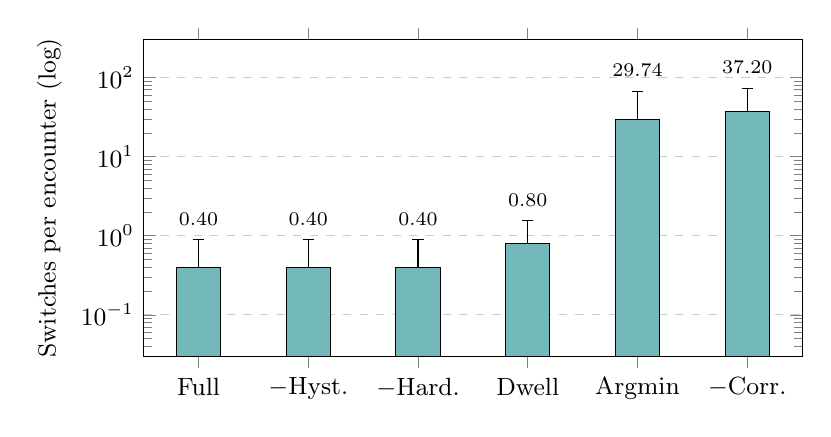
\begin{tikzpicture}
\begin{axis}[
  width=0.82\linewidth, height=5.6cm,
  ybar, bar width=16pt, ymode=log, log origin=infty,
  ymin=0.03, ymax=300,
  xtick={0,...,5}, xticklabels={{Full},{$-$Hyst.},{$-$Hard.},{Dwell},{Argmin},{$-$Corr.}},
  ylabel={Switches per encounter (log)},
  ymajorgrids, grid style={dashed,gray!40},
  error bars/y dir=plus, error bars/y explicit,
  enlarge x limits=0.1, tick label style={font=\small}, label style={font=\small},
]
\addplot[fill=teal!55, draw=black, error bars/.cd, y dir=plus, y explicit] coordinates {
(0,0.4000) +- (0,0.4909)
(1,0.4000) +- (0,0.4909)
(2,0.4000) +- (0,0.4909)
(3,0.8000) +- (0,0.7498)
(4,29.7440) +- (0,36.7008)
(5,37.2000) +- (0,36.1198)
};
\node[font=\scriptsize,anchor=south] at (axis cs:0,1.0245) {0.40};
\node[font=\scriptsize,anchor=south] at (axis cs:1,1.0245) {0.40};
\node[font=\scriptsize,anchor=south] at (axis cs:2,1.0245) {0.40};
\node[font=\scriptsize,anchor=south] at (axis cs:3,1.7823) {0.80};
\node[font=\scriptsize,anchor=south] at (axis cs:4,76.4115) {29.74};
\node[font=\scriptsize,anchor=south] at (axis cs:5,84.3178) {37.20};
\end{axis}
\end{tikzpicture}
\caption{\textbf{Class-switch count per encounter by variant} (mean with $+$SD whisker, log scale; $N=250$ per variant, 5 scenarios $\times$ 50 seeds, 10.0~s horizon), regenerated with pgfplots from \texttt{ablation\_raw.csv}. The immediate-argmin policy and the synthetic correspondence-loss stress comparator ($-$Corr.) yield 29.74 and 37.20 decision changes per encounter, respectively, whereas the proposed method (Full) maintains commitment with 0.40. Removing hysteresis ($-$Hyst.) or progress hardening ($-$Hard.) alone shows no observed regression in this scenario set, supporting the accumulator configuration's suppression of fluctuations in this scenario set; the synthetic comparator does not identify the causal effect of correspondence.}
\label{fig:oscillation}
\end{figure}


\noindent\textbf{Strongly confirmed findings.} (i) \textbf{Oscillation control (core claim).} The immediate-argmin and synthetic correspondence-loss stress comparators produce about 98 decision changes per encounter in the ambiguous-tie scenario, whereas the proposed method maintains commitment at 0 (\cref{fig:oscillation}; \cref{tab:main,tab:scenario}). The two distributions do not overlap in range (proposed method entirely 0 vs. $-$accumulator 98.16$\pm$7.85, non-overlapping observed ranges), so the observed separation is complete within these runs, not a statement about distributional support. Because the core separation in this offline measurement is categorical, a formal test would not change the conclusion, so we omit one here; Mann-Whitney U tests, effect sizes, and confidence intervals are reported for the physical performance metrics of the Planned Evaluation (\cref{app:planned}). (ii) \textbf{Spurious-input suppression.} In the transient-spike scenario, the proposed method has 0 switches (spike ignored), while argmin has 2 (entering and returning). (iii) \textbf{Rapid commitment.} In the clean-advantage scenario, the proposed method has 1 switch, with t-legible 2.37 s. (iv) \textbf{Legibility.} The oscillatory variants are frequently illegible because the posterior fails to stabilize (argmin and synthetic $-$class censoring 72/250 and 71/250, respectively; \code{near\_tie} t-legible 7.9 s vs. 0.05 s for the proposed method; \cref{tab:legibility}).

\subsection{Ablation Studies}\label{subsec:ablation}

\begin{figure}[t]
\centering
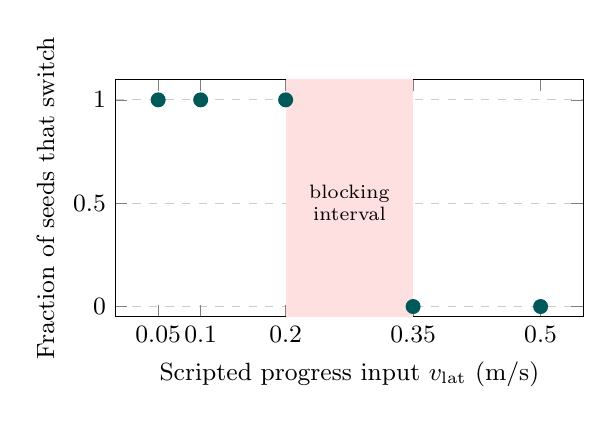
\begin{tikzpicture}
\begin{axis}[
  width=0.62\linewidth, height=4.6cm,
  xmin=0, xmax=0.55, ymin=-0.05, ymax=1.1,
  xlabel={Scripted progress input $v_{\mathrm{lat}}$ (m/s)},
  ylabel={Fraction of seeds that switch},
  xtick={0.05,0.10,0.20,0.35,0.50},
  xticklabel style={/pgf/number format/fixed, /pgf/number format/precision=2},
  ymajorgrids, grid style={dashed,gray!40},
  tick label style={font=\small}, label style={font=\small},
]
\fill[red!12] (axis cs:0.20,-0.05) rectangle (axis cs:0.35,1.1);
\node[font=\scriptsize,align=center] at (axis cs:0.275,0.5) {blocking\\interval};
\addplot[only marks, mark=*, mark size=2.5pt, teal!70!black] coordinates {(0.05,1.00) (0.10,1.00) (0.20,1.00) (0.35,0.00) (0.50,0.00)};
\end{axis}
\end{tikzpicture}
\caption{\textbf{Offline transition blocking under fast progress saturation} (\texttt{clean\_commit}, Full, 50 seeds per point, measured only at the five marked inputs; data from \texttt{R5\_rho\_sweep.md}). Every seed commits the warranted switch for $v_{\text{lat}}\le0.20$~m/s and none does for $v_{\text{lat}}\ge0.35$~m/s, so the transition-blocking interval is $v_{\text{lat}}\in(0.20,0.35)$~m/s. This is a sensitivity of the scripted progress input, not a physical freezing threshold.}
\label{fig:rhosweep}
\end{figure}


\noindent\textbf{Knob ablations: findings that diverged from the prior hypothesis (correction by measurement).} $-$Hysteresis ($\Dfloor = 0$) and $-$progress hardening ($k_\rho = 0$) showed \textbf{no observed regression} relative to the proposed method in these scenarios. Because the leaky accumulator's threshold $E_0$ and leakage already reject zero-mean noise, the primary oscillation-suppression mechanism in this operating regime is not $\Dfloor$ or $k_\rho$ but the \textbf{accumulator} itself. In other words, the earlier revision's preregistered hypothesis that ``$-$hysteresis $\to$ switch-count blowup'' does not hold under the leaky-accumulator design, and this is a \textbf{hypothesis correction} provided by the ablation measurements. In \code{intermittent}, the proposed method switches once at 1.55--2.10 s across the 50 seeds (\code{src/compass\_eval/results/README.md}) and has 0/50 censored trials, with mean t-legible 4.11 s. The earlier report of 50/50 censoring resulted from floating-point posterior saturation, not a late-horizon switch. Computing the same observer in log-odds space removes this numerical absorbing state without changing the decision policy or observer likelihood. In the same scenario, simple dwell never completes the justified switch because intermittent advantage keeps resetting the timer (0 switches), but because it remains in the initial \Class, it is immediately legible to the observer (0/50 censored, t-legible 0.05 s) --- a case where the legibility figure alone masks the switching failure. Simple dwell's total censoring (50/50) occurs not in \code{intermittent} but in \code{mid\_reversal} (after the mid-course switch, the posterior fails to re-stabilize by the end of the horizon), whereas in the same scenario the proposed method maintains commitment (0 switches) and is immediately legible with 0/50 censoring. However, the proposed method's zero switches in \code{mid\_reversal} is the flip side of this same masking effect --- at the default knobs, the accumulator fails to track a late-horizon reversal (in the scenario script, the challenger advantage rises to $+0.25$, i.e., $5\times\Dfloor$, by the end of the horizon; verified at \code{harness.hpp:56}), which is consistent with the conservatism cost noted in \cref{subsec:switch} and the offline transition-blocking sensitivity measured below. \Cref{prop:p2live} makes this quantitative rather than a masking artefact: at the default knobs a discretionary switch at $\rho = 0$ is reachable only for a sustained advantage exceeding $0.23$ (\cref{rem:resptime}), and even at $D_{\text{sus}} = 0.25$ the response-time bound is $N_{\text{resp}} = 76$ cycles ($3.8$ s); the scenario's advantage ramps linearly from $-0.25$ to $+0.25$ over the $10$ s horizon, so it exceeds $0.23$ only in the final $8$ cycles ($0.4$ s), and driving the noiseless ramp through the leaky recursion leaves $\Erev \approx 0.21 < E_0$ at the end of the horizon. The measured $0$ switches is therefore what the analysis predicts for this scenario at these knobs, and the open question it leaves is a knob-design one (a lower $E_0$ improves responsiveness at the cost of the P2 margin; increasing $\lambda$ reduces leak but leaves the stated P2 lower bound unchanged), not a hidden failure of the mechanism. Finally, the t-legible and censoring-rate figures in this section, obtained from the decision-stream proxy observer of \cref{subsec:setup}, measure the stability of the decision stream, not an independent axis of motion legibility, as already noted.

\noindent\textbf{$\rho$-rate sensitivity and offline transition blocking.} The effect of progress hardening depends strongly on the $\rho$ drive rate. Measuring in the scripted \code{clean\_commit} decision-core harness while raising its progress input $v_{\text{lat}}$ from 0.05 to 0.50 m/s, the proposed method always commits (\cref{fig:rhosweep}) (50/50, t-legible $\approx$ 2.4 s) for $v_{\text{lat}} \le 0.20$ m/s, but \textbf{switching is blocked (0/50) for $v_{\text{lat}} \ge 0.35$ m/s}. This is because a rapidly saturating $\rho$ raises $\Eth$ to $E_0(1+k_\rho) = 0.60$, blocking even justified switches --- the clip obstruction in \Cref{prop:p2live} gives a noise-independent blocking mechanism: with the scenario's advantage of $+0.40$ the leak equilibrium is $(0.40-\Dfloor)\,dt/(1-\lambda) = 0.583 < 0.60$, in the noiseless constant-advantage model; independently, the clip bound $e_{\max}=0.50<0.60$ blocks every discretionary switch after saturation regardless of noise, whereas at $\rho = 0$ the same advantage switches within $N_{\text{resp}} = 24$ cycles ($1.2$ s). Whether the switch wins the race against the rising threshold before saturation is precisely what the sweep measures; the \textbf{offline transition-blocking interval is $v_{\text{lat}} \in (0.20, 0.35)$ m/s}. This is a sensitivity of the scripted input and the core's former simplification $v_{\text{lat}}=|v_{\text{cmd}}|$; it does not demonstrate robot immobility, physical freezing, or goal failure. It motivates separating measured cross-track progress from forward speed (\code{compass\_eval/results/R5\_rho\_sweep.md}).

\subsection{Real-Time Performance and Enumeration Complexity}\label{subsec:latency}

\begin{table}[t]
\centering
\caption{\textbf{Historical decision-core timing} of \texttt{DecisionCore::step} (enumeration, cost integration, safety test and decision), 20{,}000 iterations per condition on an AMD Ryzen 5 5500GT, all $2^K$ labels enumerated in an all-safe fixture. Finite-batch measurements, not a worst-case execution-time bound and not an end-to-end ROS~2 pipeline measurement.}
\label{tab:latency}
\small
\begin{tabular}{ccrrrrr}
\toprule
$K$ & Labels $2^K$ & Mean ($\mu$s) & p50 ($\mu$s) & p99 ($\mu$s) & Max ($\mu$s) & Max / 50 ms \\
\midrule
1 & 2 & 1.6 & 1.5 & 2.6 & 153.6 & 0.31\% \\
2 & 4 & 5.4 & 5.2 & 7.9 & 356.1 & 0.71\% \\
3 & 8 & 15.9 & 14.5 & 58.6 & 651.3 & 1.30\% \\
\bottomrule
\end{tabular}
\end{table}


\noindent\textbf{Enumeration complexity (analytical bound).} The current core enumerates $2^K$ labels with $K=\min(N_{\rm people},K_{\rm cap})$ and evaluates each candidate before forming its safe set. At the default $K_{\rm cap}=3$, that is at most eight labels. This is a configured enumeration bound, not evidence that influence ranking, coarse group merging, or a particular pruning distribution has been implemented. The cost of each evaluation also depends on rollout samples, people, and environment queries; the distribution of the resulting $|\mathcal{S}_k|$ in physical scenes remains unmeasured. The ideal pruning/lifecycle design in \cref{subsec:enum} is not a reason to treat the present loop as evaluating only already-safe classes.

\noindent\textbf{$K_{\text{cap}}$ operating rule.} The current implementation retains the first $K_{\rm cap}$ people in input order as explicit class dimensions, with default value 3. It does not compute an influence ranking or merge overflow people into coarse classes. Input selection and ordering therefore matter. Person-cost and safety queries can still examine the supplied people beyond those label dimensions, but that is not a guarantee of a realized passing-side relationship for them.

\noindent\textbf{Historical finite-batch timing.} The archived \code{compass\_eval latency} experiment measured \code{DecisionCore::step} on an AMD Ryzen 5 5500GT with Radeon Graphics for 20,000 iterations per condition, using all $2^K$ enumerated labels and an all-safe environment fixture. The observed p99/max pairs (\cref{tab:latency}) are 2.6/153.6 $\mu$s at $K=1$, 7.9/356.1 $\mu$s at $K=2$, and 58.6/651.3 $\mu$s at $K=3$. The largest observed maximum is about 1.30\% of a 50 ms (20 Hz) period. These are finite-batch measurements, not a proven worst-case execution-time (WCET) bound or an upper bound on deployment latency. The loop evaluates the enumerated candidates before constructing $\mathcal{S}_k$; its work also depends on all supplied people, rollout samples, and environment-query costs, not only $|\mathcal{S}_k|$. Limiting explicit label dimensions does not independently bound all these costs. This historical measurement does not benchmark the new candidate adapter, live costmap access or the end-to-end ROS 2 pipeline (callbacks, TF, controller dispatch, DDS/executor jitter). Those timings and the physical-scene safe-set distribution remain separate evaluation targets.
